\section{Web Entry Server}
Ein \textit{Web Entry Server} ist ein Reverse Proxy mit WAF Filtermöglichkeiten und zentral gesteuerten Authentication- / Authorization-Services, um den Zugang zu Web Applikationen zu steuern. Ohne \textit{WES} wären alle Applikationen durch Verbindungen in die DMZ direkt erreichbar.

\begin{figure}[H]
	\centering
	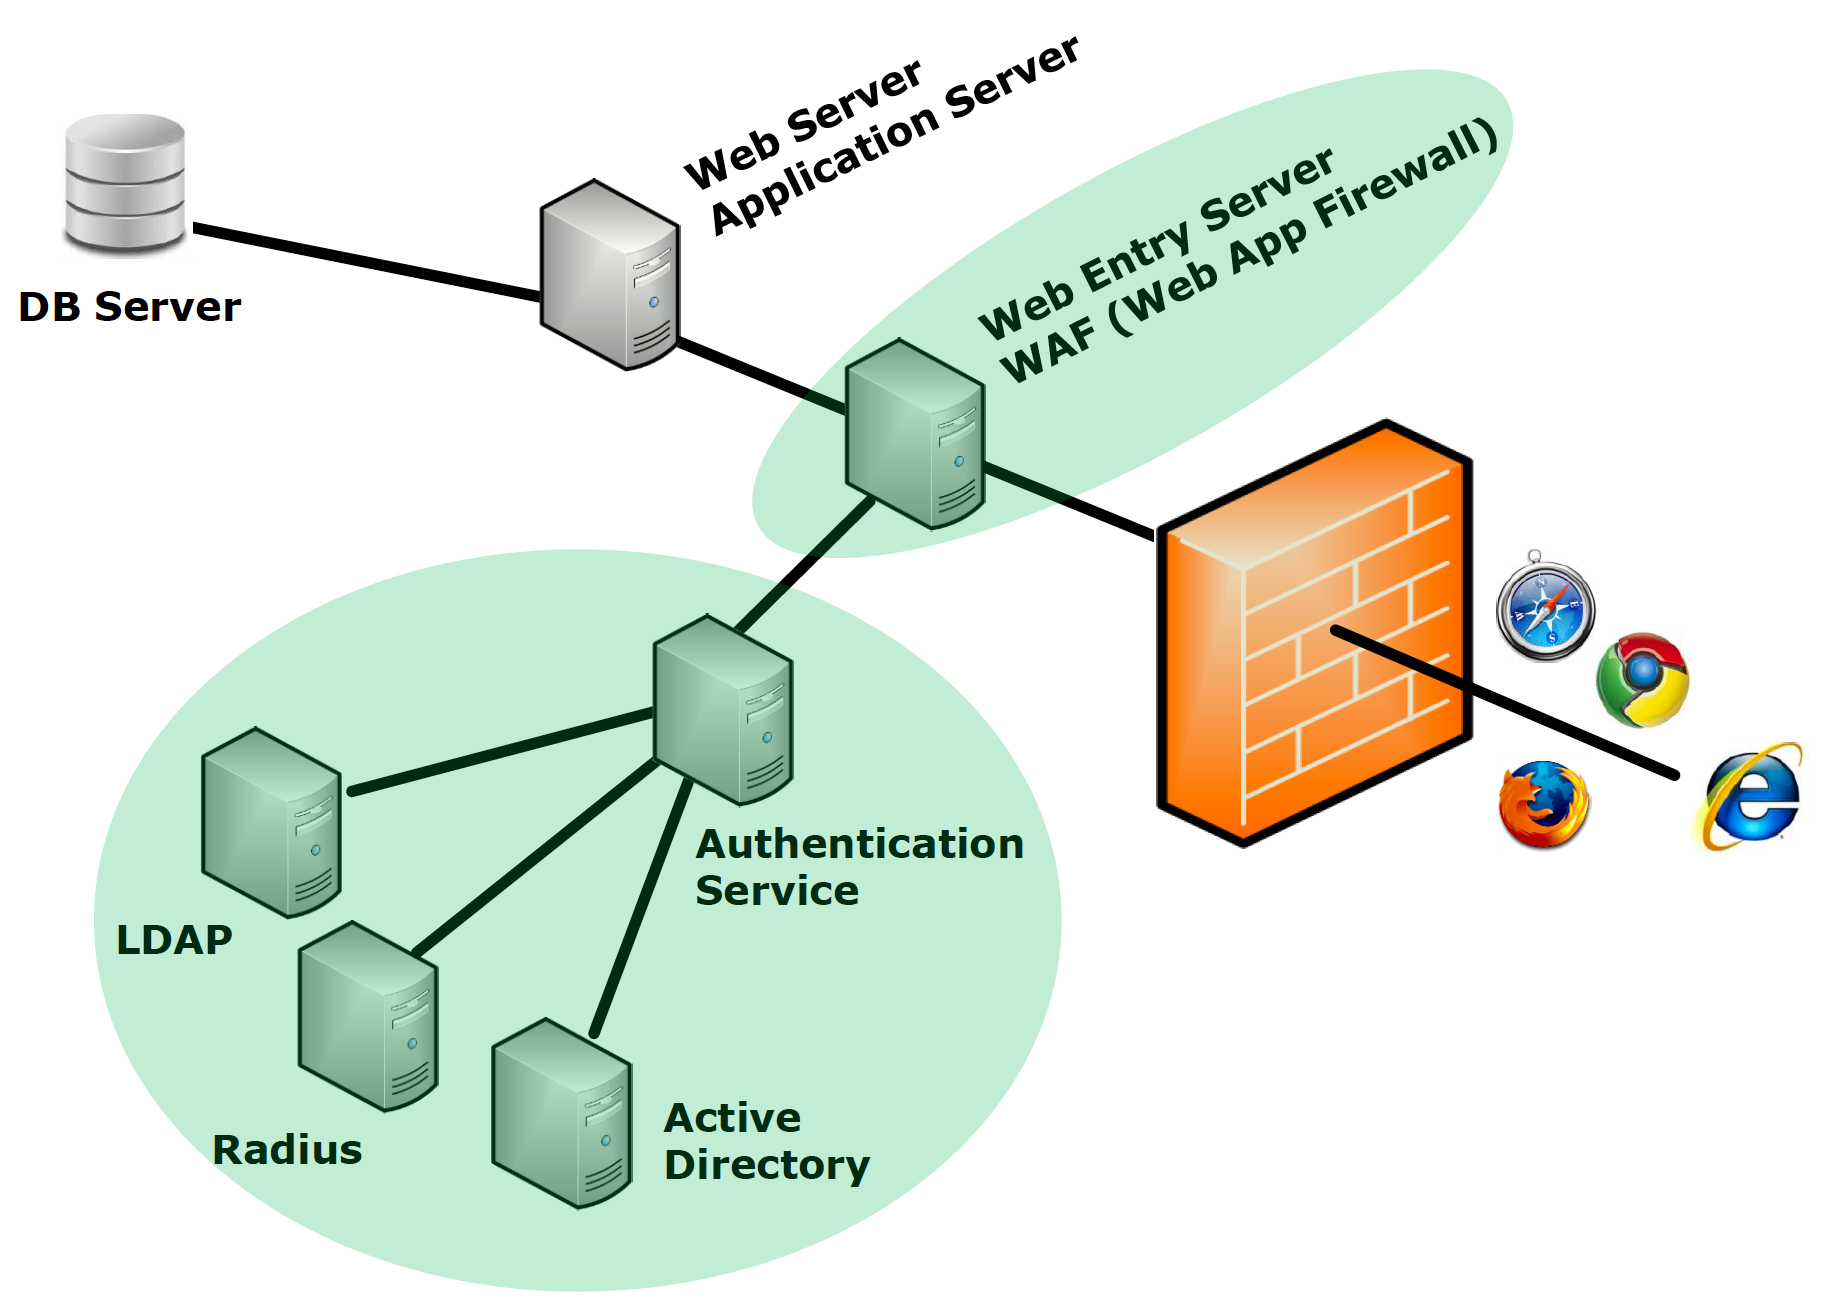
\includegraphics[width=0.7\textwidth]{./img/web-entry-server-schema}
	\caption{Beispielschema eines Netzwerks mit Web Entry Server}
\end{figure}

Üblicherweise wir dieser als modifizierter Apache Web Server implementiert und kann folgende Funktionen übernehmen:

\begin{easylist}[itemize]
	& Network Filter Level
	& SSL Termination
	& Protocol Validation and Rebuilding
	& Character Encoding and Unicode Verficatoin
	& White / Black List Filter
	& Cookie Protection
	& URL Encrypting
	& Smart Form Protection
	& Response Content Filter
	& Response Rewriting
	& Pre-Authentication
\end{easylist}

\subsection{Reverse Proxy}
Ein Reverse Proxy lädt Ressourcen für einen Client von mehreren Servern. Die Adressen der Zielsysteme bleiben für den Client dabei verborgen.
Modul: \textbf{mod\_proxy}

\subsection{Pre-Authentication}
Der Zweck einer Pre-Authentication ist, dass jegliche \textbf{Backend Requests} bereits \textbf{authentifiziert} sind. Dies bietet zudem fortgeschrittene Logging- und Forensik-Möglichkeiten.

\subsubsection{Ablauf}
\begin{easylist}[enumerate]
	& Anfrage des Clients an die App wird zu Login Server weitergeleitet
	& Client erhält Cookie für Authentifizierungsprozess
	& Bei erfolgreichem Login erhält der Client ein neues Cookie
	& Client verwendet Cookie für Zugriff auf Applikation
\end{easylist}

\subsubsection{Zweck der Cookies}
Bei den Cookies muss jeweils ein Zeitstempel und eine Zufallszahl (Nonce) enthalten sein, um \textbf{Replay Attacken} zu verhindern.\\

Das zweite Cookie nach erfolgreicher Authentifizierung wird benötigt, um gegen \textbf{Session Fixation} zu wirken. Bei dieser Attacke bringt der Angreifer einen Benutzer dazu, sich mit seiner Session ID zu authentifizieren, welcher dann Zugriff auf die Applikation erhält.\\
\textbf{Modul: mod\_but}

\subsection{Filtering}
Der Web Entry Server übernimmt das Herausfiltern von unerwünschten Requests (z.B. SQL Injections) und Responses (z.B. Stack Traces).\\
\textbf{Modul: mod\_security}

\subsection{Unique ID}
Dank Generierung und Weiterleitung einer Unique ID innerhalb aller Systeme lassen sich die verschiedenen Logfiles miteinander korrelieren. Man spricht dabei von der \textbf{Forensic Readiness}.\\
\textbf{Module: mod\_unique\_id, mod\_headers}.

\subsection{URL Encryption}
Bei der URL-Encryption wird die URL dynamisch verschlüsselt, um gegen manipulierte URLs (\textbf{Forceful Browsing}) zu kämpfen, um \textbf{Parameter zu schützen}, und \textbf{Technologie und Topologie} zu verstecken.

\subsection{Content Rewriting}
Relative URLs sind generell kein Problem. Absolute URLs, die Cookie Domain und in manchen Fällen die Werte der Cookies müssen jedoch ersetzt werden.\\
\textbf{Modul: mod\_substitute}

\subsection{Session Store}
Falls Anpassungen der Cookies bei einer Anwendung nicht möglich sind (HttpOnly, Secure), kann die WAF hier einspringen. Sie weist dem Client eine ID zu und speichert selbst alle Session-Cookies der Anwendung, anstatt sie an den Client weiterzuleiten. Bei einer Anfrage reichert die WAF diese wieder mit dem passenden Session-Cookie an. Die Session-ID des Clients kann somit mit weiteren Client-Eigenschaften verglichen werden (\textbf{Sticky Sessions}). Auch ermöglicht dies die zentrale Verwaltung von Sessions, z.B. \textbf{Session Expiration}.